\begin{proof}
Consider the case where $\lambda/\mu$ consists of only those four columns $c_1,c_2,c_3,c_4$. Without loss of generality say $\{c_1,c_2\} = \{3,4\}$ and $\CS _{c_1}(\lambda/\mu)<\CS _{c_2}(\lambda/\mu)$, and $\{c_3,c_4\} = \{1,2\}$ with $\CS _{c_3}(\lambda/\mu)<\CS _{c_4}(\lambda/\mu)$. There are four possible arrangements of $c_1$ through $c_4$ as shown in Figure~\ref{only4col}. Let $\rho_i \coloneqq \CS _{c_i}(\lambda/\mu)$ for $i \in \{1,2,3, 4\}$.

\begin{figure}[htb]\centering
 % \begin{center}
 \begin{subfigure}{0.24\textwidth}
 \hspace{0.5cm}
 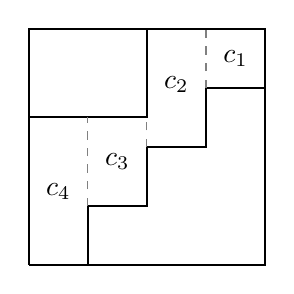
\begin{tikzpicture}[scale = 0.75]
 \draw[black, thick] (0,0) -- (4,0) -- (4,4) -- (0,4) -- (0,0);
 \draw[black, thick] (1,0) -- (1,1) -- (2,1) -- (2,2) -- (3,2) -- (3,3) -- (4,3);
 \draw[black, thick] (0,2.5) -- (2,2.5) -- (2,4);
 \draw[gray, dashed] (1,1) -- (1,2.5);
 \draw[gray, dashed] (3,3) -- (3,4);
		\draw[gray, dashed] (2,2) -- (2,2.5);
 \draw (3.5,3.5) node{$c_1$};
 \draw (2.5,3.05) node{$c_2$};
 \draw (1.5, 1.75) node{$c_3$};
 \draw (0.5, 1.25) node{$c_4$};
 \end{tikzpicture}
 \caption{}
	\label{Figure2a}
 \end{subfigure}
 \begin{subfigure}{0.24\textwidth}
 \hspace{0.6cm}
 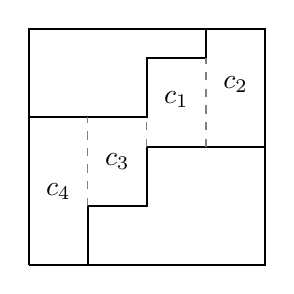
\begin{tikzpicture}[scale=0.75]
 \draw[black, thick] (0,0) -- (4,0) -- (4,4) -- (0,4) -- (0,0);
 \draw[black, thick] (1,0) -- (1,1) -- (2,1) -- (2,2) -- (4,2);
 \draw[black, thick] (0,2.5) -- (2,2.5) -- (2,3.5) -- (3,3.5) -- (3,4);
 \draw[gray, dashed] (1,1) -- (1,2.5);
 \draw[gray, dashed] (3,2) -- (3,3.5);
			\draw[gray, dashed] (2,2) -- (2,2.5);
 \draw (3.5,3.05) node{$c_2$};
 \draw (2.5,2.8) node{$c_1$};
 \draw (1.5,1.75) node{$c_3$};
 \draw (0.5,1.25) node{$c_4$};
 \end{tikzpicture}
 \caption{}
 \end{subfigure}
 \begin{subfigure}{0.24\textwidth}
 \hspace{0.7cm}
 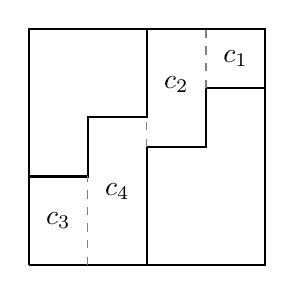
\begin{tikzpicture}[scale=0.75]
 \draw[black, thick] (0,0) -- (4,0) -- (4,4) -- (0,4) -- (0,0);
 \draw[black, thick] (2,0) -- (2,2) -- (3,2) -- (3,3) -- (4,3);
 \draw[black, thick] (0,1.5) -- (1,1.5) -- (1,2.5) -- (2,2.5) -- (2,4);
 \draw[gray, dashed] (1,0) -- (1,1.5);
 \draw[gray, dashed] (3,3) -- (3,4);
			\draw[gray, dashed] (2,2) -- (2,2.5);
 \draw (3.5,3.5) node{$c_1$};
 \draw (2.5,3.05) node{$c_2$};
 \draw (1.5,1.25) node{$c_4$};
 \draw (0.5,0.75) node{$c_3$};
 \end{tikzpicture}
 \caption{}
 \end{subfigure}
 \begin{subfigure}{0.24\textwidth}
 \hspace{0.75cm}
 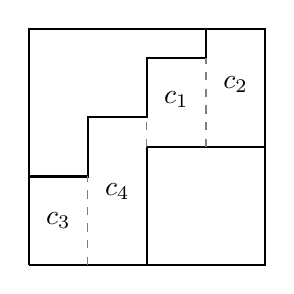
\begin{tikzpicture}[scale=0.75]
 \draw[black, thick] (0,0) -- (4,0) -- (4,4) -- (0,4) -- (0,0);
 \draw[black, thick] (2,0) -- (2,2) -- (4,2);
 \draw[black, thick] (0,1.5) -- (1,1.5) -- (1,2.5) -- (2,2.5) -- (2,3.5) -- (3,3.5) -- (3,4);
 \draw[gray, dashed] (1,0) -- (1,1.5);
 \draw[gray, dashed] (3,2) -- (3,3.5);
			\draw[gray, dashed] (2,2) -- (2,2.5);
 \draw (3.5,3.05) node{$c_2$};
 \draw (2.5,2.8) node{$c_1$};
 \draw (1.5,1.25) node{$c_4$};
 \draw (0.5,0.75) node{$c_3$};
 \end{tikzpicture}
 \caption{}
		\label{Figure2d}
 \end{subfigure}
 \caption{}
 \label{only4col} 
% \end{center}
\end{figure}

We want to construct two distinct ballot fillings of $\lambda/\mu$ with the same content. In both fillings, we fill column $c_1$ and $c_2$ with $[\rho_1]$ and $[\rho_2]$ respectively. The entries of column $c_3$ and $c_4$ depend on the relative sizes of $\rho_1,\rho_2,\rho_3,\rho_4$ and the relative sizes of $c_3$ and $c_4$.


\begin{Case}
%\noindent \emph
{\hypertargeta{prop3.7case_1}{Case 1} $(c_3 > c_4$, $\rho_2\geq \rho_4$, $\rho_4-1\geq \rho_1+1$, $\rho_3\geq \rho_1)$} 
For Filling 1, fill column $c_3$ with $[\rho_3+1]\setminus \{\rho_1\}$ and column $c_4$ with $([\rho_4]\setminus\{\rho_3+1\})\cup\{\rho_2+1\}$.
For Filling 2, fill column $c_3$ with $([\rho_3]\setminus \{\rho_1\})\cup \{\rho_2+1\}$ and column $c_4$ with $[\rho_4]$.
\end{Case}

\begin{Case}
%\noindent \emph
{\hypertargeta{prop3.7case_2}{Case 2} $(c_3 > c_4$, $\rho_2\geq \rho_4$, $\rho_4-1\geq \rho_1+1$, $\rho_3< \rho_1)$} 
For Filling 1, fill column $c_3$ with $[\rho_3-1]\cup \{\rho_1 + 1\}$ and column $c_4$ with $([\rho_4]\setminus\{\rho_1+1\})\cup\{\rho_2+1\}$.
For Filling 2, fill column $c_3$ with $[\rho_3-1]\cup \{\rho_2+1\}$ and column $c_4$ with $[\rho_4]$.
\end{Case}

\begin{Case}
%\noindent \emph
{\hypertargeta{prop3.7case_3}{Case 3} $(c_3 > c_4$, $\rho_2\geq \rho_4$, $\rho_4-1< \rho_1+1)$} 
For Filling 1, fill column $c_3$ with $[\rho_3-1]\cup \{\rho_1+1\}$ and column $c_4$ with $[\rho_4-1]\cup \{\rho_2+1\}$. For Filling 2, fill column $c_3$ with $[\rho_3-1]\cup \{\rho_2+1\}$ and column $c_4$ with $[\rho_4-1]\cup \{\rho_1+1\}$.
\end{Case}

\begin{Case}
%\noindent \emph
{\hypertargeta{prop3.7case_4}{Case 4} $(c_3> c_4$, $\rho_2< \rho_4$, $\rho_3\geq \rho_2)$} 
For Filling 1, fill column $c_3$ with $[\rho_3+1]\setminus\{\rho_1\}$ and column $c_4$ with $[\rho_4+1]\setminus \{\rho_2\}$. For Filling 2, fill column $c_3$ with $[\rho_3+2]\setminus \{\rho_1,\rho_2\}$ and column $c_4$ with $[\rho_4+1]\setminus \{\rho_3+2\}$.
\end{Case}

\begin{Case}
%\noindent \emph
{\hypertargeta{prop3.7case_5}{Case 5} $(c_3 > c_4$, $\rho_2< \rho_4$, $\rho_3< \rho_2$, $\rho_1\geq \rho_3)$} 
For Filling 1, fill column $c_3$ with $[\rho_3 -1 ]\cup \{\rho_1+1\}$ and column $c_4$ with $[\rho_4+1]\setminus \{\rho_1+1\}$. For Filling 2, fill column $c_3$ with $[\rho_3 -1 ]\cup \{\rho_2+1\}$ and column $c_4$ with $[\rho_4+1]\setminus \{\rho_2+1\}$.
\end{Case}

\begin{Case}
%\noindent 
\emph{\hypertargeta{prop3.7case_6}{Case 6} $(c_3 > c_4$, $\rho_2< \rho_4$, $\rho_3< \rho_2$, $\rho_1< \rho_3)$} 
For Filling 1, fill column $c_3$ with $[\rho_3+1]\setminus \{\rho_1\}$ and column $c_4$ with $[\rho_4+1]\setminus \{\rho_3+1\}$. For Filling 2, fill column $c_3$ with $([\rho_3]\setminus \{\rho_1\})\cup\{\rho_2+1\}$ and column $c_4$ with $[\rho_4+1]\setminus \{\rho_2+1\}$.
\end{Case}

\begin{Case}
%\noindent \emph
{\hypertargeta{prop3.7case_7}{Case 7} $(c_3 < c_4$, $\rho_2\geq \rho_4$, $\rho_4-1 < \rho_1+1)$} 
For Filling 1, fill column $c_3$ with $[\rho_3-1]\cup \{\rho_1+1\}$ and column $c_4$ with $[\rho_4-1]\cup \{\rho_2+1\}$. For Filling 2, fill column $c_3$ with $c_3$ with $[\rho_3-1]\cup \{\rho_4-1\}$ and column $c_4$ with $[\rho_4-2]\cup \{\rho_1+1,\rho_2+1\}$.
\end{Case}

\begin{Case}
%\noindent \emph
{\hypertargeta{prop3.7case_8}{Case 8} $(c_3 < c_4$, $\rho_2\geq \rho_4$, $\rho_4-1 \geq \rho_1+1$, $\rho_1\geq \rho_3)$} 
For Filling 1, fill column $c_3$ with $[\rho_3-1]\cup \{\rho_1\}$ and column $c_4$ with $([\rho_4]\setminus\{\rho_1\}\cup \{\rho_2+1\}$. For Filling 2, fill column $c_3$ with $[\rho_3-1]\cup \{\rho_4\}$ and column $c_4$ with $[\rho_4-1]\cup \{\rho_2+1\}$.
\end{Case}

\begin{Case}
%\noindent \emph
{\hypertargeta{prop3.7case_9}{Case 9} $(c_3 < c_4$, $\rho_2\geq \rho_4$, $\rho_4-1 \geq \rho_1+1$, $\rho_1< \rho_3)$} 
For Filling 1, fill column $c_3$ with $([\rho_3]\setminus \{\rho_1\})\cup \{\rho_4\}$ and column $c_4$ with $[\rho_4-1]\cup \{\rho_2+1\}$.
For Filling 2, fill column $c_3$ with $[\rho_3]$ and column $c_4$ with $([\rho_4]\setminus\{\rho_1\})\cup \{\rho_2+1\}$.
\end{Case}

\begin{Case}
%\noindent \emph
{\hypertargeta{prop3.7case_10}{Case 10} $(c_3 < c_4$, $\rho_2< \rho_4$, $\rho_2 \leq \rho_3)$} 
For Filling 1, fill column $c_3$ with $[\rho_3+1]\setminus \{\rho_1\}$ and column $c_4$ with $[\rho_4+1]\setminus \{\rho_2\}$. For Filling 2, fill column $c_3$ with $[\rho_3+1]\setminus \{\rho_2\}$ and column $c_4$ with $[\rho_4+1]\setminus \{\rho_1\}$.
\end{Case}

\begin{Case}
%\noindent \emph
{\hypertargeta{prop3.7case_11}{Case 11} $(c_3 < c_4$, $\rho_2< \rho_4$, $\rho_2 > \rho_3$, $\rho_3>\rho_1)$} 
For Filling 1, fill column $c_3$ with $([\rho_3]\setminus \{\rho_1\})\cup \{\rho_2\}$ and column $c_4$ with $[\rho_4+1]\setminus \{\rho_2\}$. For Filling 2, fill column $c_3$ with $[\rho_3]$ and column $c_4$ with $[\rho_4+1]\setminus \{\rho_1\}$.
\end{Case}

\begin{Case}
%\noindent \emph
{\hypertargeta{prop3.7case_12}{Case 12} $(c_3 < c_4$, $\rho_2< \rho_4$, $\rho_2 > \rho_3$, $\rho_3\leq\rho_1)$} 
For Filling 1, fill column $c_3$ with $[\rho_3-1]\cup \{\rho_1\}$ and column $c_4$ with $[\rho_4+1]\setminus \{\rho_2\}$. For Filling 2, fill column $c_3$ with $[\rho_3-1]\cup \{\rho_2\}$ and column $c_4$ with $[\rho_4+1]\setminus \{\rho_1\}$.
\end{Case}

In all of the above cases, both fillings have the same content, and they are strictly increasing within columns. Similarly, in all cases the column reading word is ballot. It remains to show that the fillings are weakly increasing within rows.

For each pair of indices $(c_1,c_2)$ or $(c_3,c_4)$, the fillings described above are weakly increasing within rows for those column pairs. Let $c'' = \max\{c_3,c_4\}$ and $c' = \min \{c_1,c_2\}$. It remains to show that the fillings described above are weakly increasing within rows for the column pair $c'$ and $c''$.

\begin{claim}
\label{claim:col2col3}
Let $T$ be any one of the fillings defined in the twelve cases above. If $(r,c''),(r,c')\in \lambda/\mu$, then $T(r,c'') \leq T(r,c')$.
\end{claim}

\begin{proof}
Let $\rho'' = \CS _{c''}(\lambda/\mu)$. Because $U(c'')>U(c')$ and $\CS _{c'}(\lambda/\mu)\leq \rho_2$, at most the top $\rho_2-1$ boxes of column $c''$ are to the left of a box in column $c'$. In addition, the boxes in column $c'$ have at least one more box above them than the corresponding box in column $c''$. Similarly, because $L(c'')>L(c')$, at most the top $\rho''-1$ boxes of column $c''$ are to the left of a box in column $c'$. Combining these two facts, we know that at most the top $\min(\rho_2,\rho'')-1$ boxes in column $c''$ have a box in $c'$ directly to the right of it.

Observe that in nearly all of the cases above, for $1\leq k\leq \min(\rho_2,\rho'')-1$, the $k^{th}$ box from the top of column $c''$ has an entry of at most $k+1$, and its right neighbor has at least $k$ boxes above it. Even if column $c'$ was minimally filled, its entries would still be at least the value of the corresponding entries in column $c''$. This proves the claim in these cases.

There are only two exceptions to the above observation: \hyperlinka{prop3.7case_4}{Case 4} and \hyperlinka{prop3.7case_7}{Case 7}.

In \hyperlinka{prop3.7case_4}{Case 4}, the only box contradicting the observation is the box that is $\rho_2-1$ from the top of column $c''=c_3$, which has value $\rho_2+1$. This would violate semistandardness if and only if
\begin{equation}
\label{eq:zz1010}
c'=c_2\text{ and }U(c_2) = U(c_3)-1.
\end{equation}
In this case $\mu$ is a rectangle of shortness 1, and thus~\eqref{eq:zz1010} cannot be satisfied.

In \hyperlinka{prop3.7case_7}{Case 7}, the only box contradicting the observation is the box that is $\rho_4-1$ from the top of column $c''=c_4$, which has value $\rho_1+1$. This would violate semistandardness if and only if
\begin{equation}
\label{eq:zz2020}
c'=c_1\text{ and }L(c_1) = L(c_4)-1.
\end{equation}
In this case $\lambda^\vee$ is a rectangle of shortness 1, and thus~\eqref{eq:zz2020} cannot be satisfied.

As a result, in all cases, both fillings of $\lambda/\mu$ are semistandard.
\end{proof}

This completes the proof in the case where $\lambda/\mu$ consists of exactly four columns. If $\lambda/\mu$ has more than four columns, then let $\lambda^*/\mu^*$ be the skew shape consisting of the four columns in the statement of the theorem. If neither $(\lambda^*)^\vee$ nor $\mu^*$ is a rectangle of shortness $1$, then we have shown that $s_{\lambda^*/\mu^*}(x_1,\dots, x_{\rho(\lambda^*/\mu^*) + 1})$ is not multiplicity-free. By Corollary~\ref{Cor:GUT2}, $s_{\lambda^*/\mu^*}(x_1,\dots, x_{\rho(\lambda^*/\mu^*) + 1})$ is not multiplicity-free implies $s_{\lambda/\mu}(x_1,\dots, x_{\rho(\lambda/\mu) + 1})$ is not multiplicity-free.

On the other hand, suppose either $(\lambda^*)^\vee$ or $\mu^*$ is a rectangle of shortness $1$ as in Figure~\ref{Figure2a} or Figure~\ref{Figure2d}. Since neither $\lambda^\vee$ nor $\mu$ is a rectangle of shortness $1$, there must exist some other column $c$ such that $U(c),U(c_i),U(c_j)$ are all distinct, and $L(c),L(c_i),L(c_j)$ are all distinct for some $1\leq i<j\leq 4$. By Proposition~\ref{prop:3col}, $s_{\lambda/\mu}(x_1,\dots, x_{\rho(\lambda/\mu)+1})$ is not multiplicity-free.
\end{proof}
